
\begin{figure}[hp]
\centering
% 
    \begin{subfigure}[t]{.5\linewidth}
    \centering
    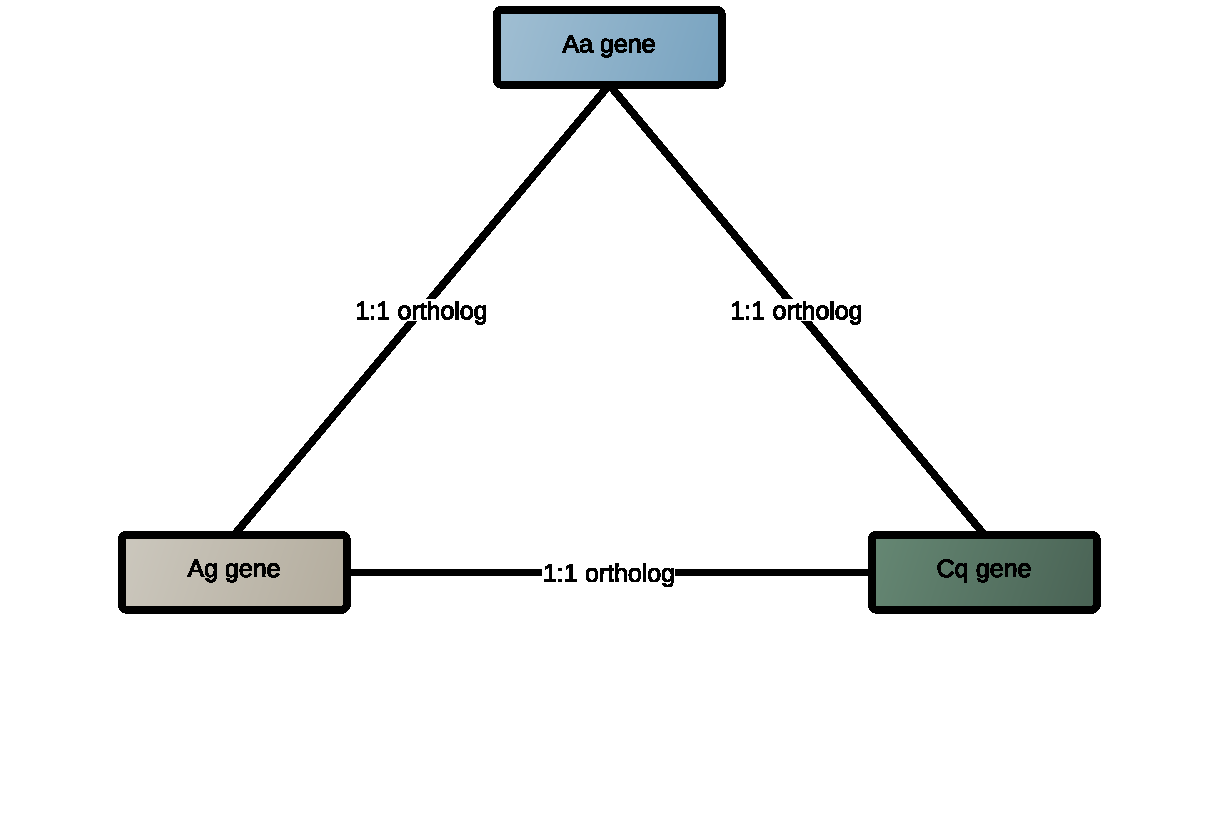
\includegraphics[width=\linewidth]{figures/figs/gfunc_graph_figs/ortho-graph-model.pdf}
    \caption{N-way 1:1 ortholog graph structure}\label{fig:nway-ortholog-graph-model}
    \end{subfigure}%
% 
% 
% 
    \begin{subfigure}[t]{.5\linewidth}
    \centering
    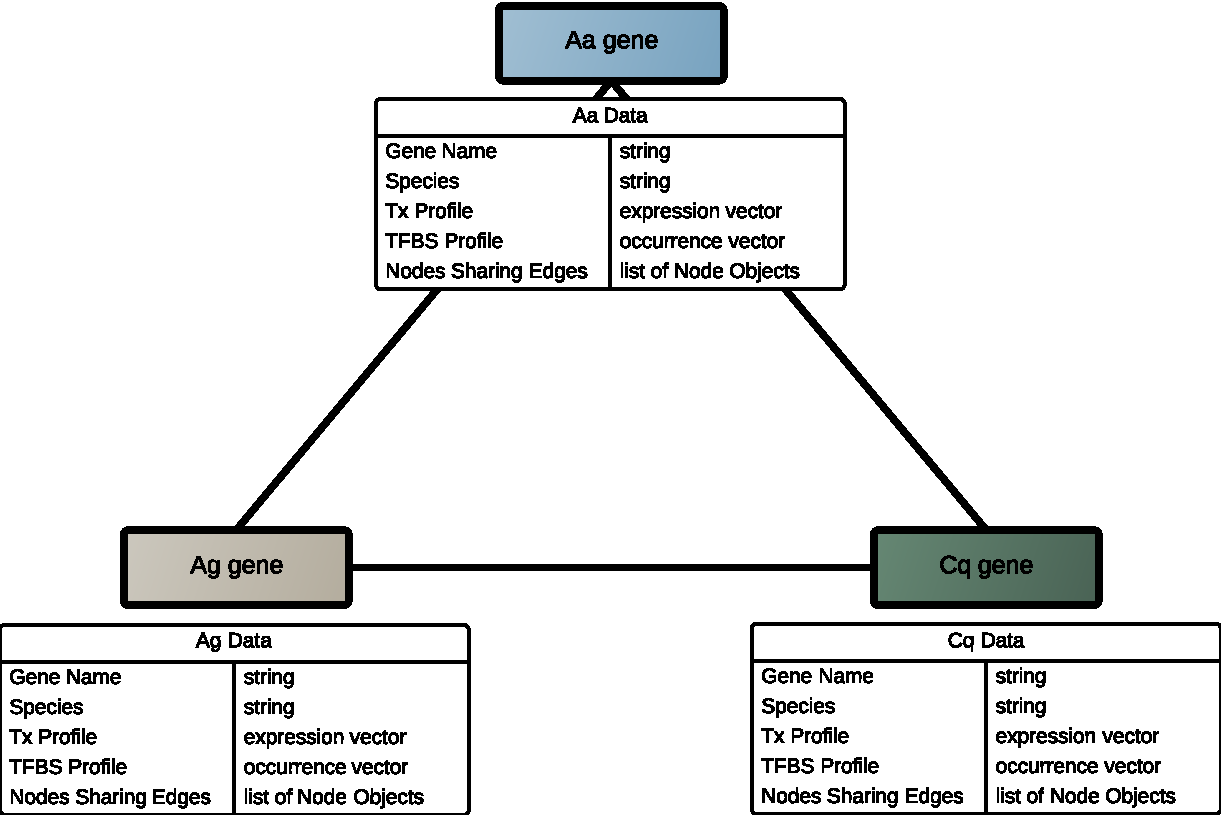
\includegraphics[width=\linewidth]{figures/figs/gfunc_graph_figs/ortho-graph-node-data.pdf}
    \caption{Node data model}\label{fig:nway-ortholog-graph-node-data}
    \end{subfigure}
% 
% 
% 
% 
% 
% 
    \begin{subfigure}[t]{.5\linewidth}
    \centering
    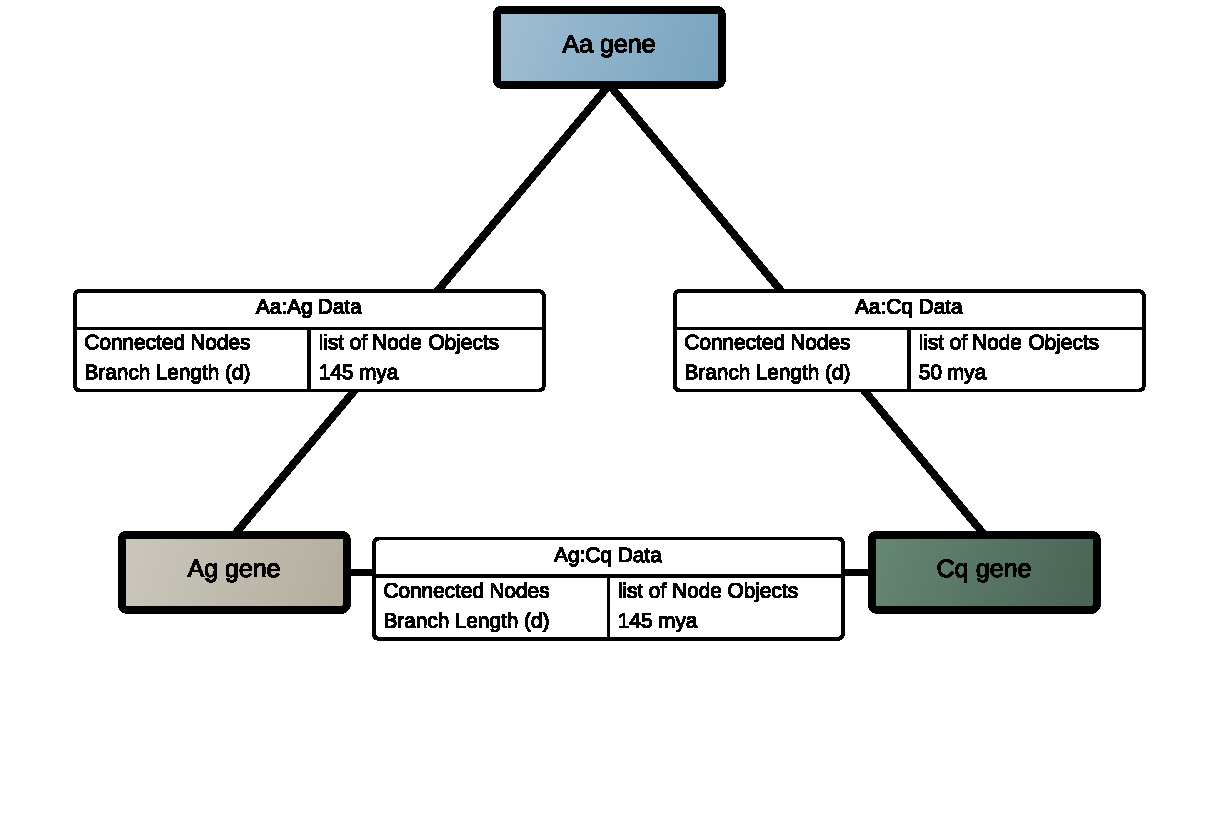
\includegraphics[width=\linewidth]{figures/figs/gfunc_graph_figs/ortho-graph-edge-data.pdf}
    \caption{Edge data model}\label{fig:nway-ortholog-graph-edge-data}
    \end{subfigure}%
% 
% 
%     
    \begin{subfigure}[t]{.5\linewidth}
    \centering
    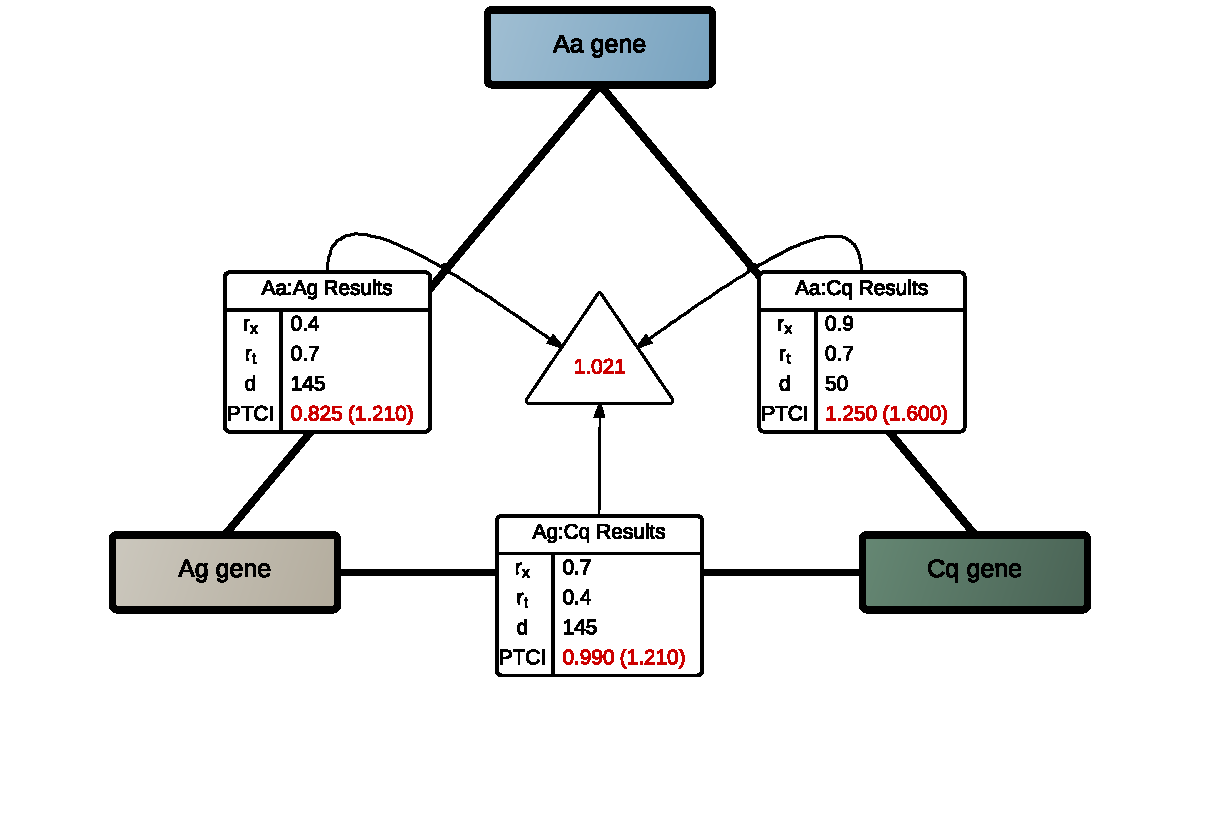
\includegraphics[width=\linewidth]{figures/figs/gfunc_graph_figs/ortho-graph-ptci.pdf}
    \caption{Example PTCI data}\label{fig:nway-ortholog-graph-ptci}
    \end{subfigure}
% 
% 
% 
\caption[Graph model used to integrate data types]{\sf \textbf{Graph model used to integrate data types.}}\label{fig:nway-ortholog-graph}
\end{figure}